\documentclass[a4paper,12pt]{article}

\usepackage{graphicx}
\usepackage{amsmath}
\usepackage{siunitx}
\sisetup{per-mode=symbol,exponent-product=\cdot,range-phrase=\ldots}
\usepackage{tikz,pgfplots}
\pgfplotsset{compat=1.18}
\usepackage{titlesec}
\usepackage{enumitem}
\usepackage{tex/ET_Ueb_Header_2Ebenen}

\graphicspath{{./}{./templates/}}

\renewcommand\thesection{\Alph{section}}
\titleformat{\section}[hang]{\normalfont\Large\bfseries}{Aufgabe \thesection)}{.8em}{}
\renewcommand\thesubsection{\thesection.\arabic{subsection}}
\titleformat{\subsection}[hang]{\normalfont\large\bfseries}{Teil \thesubsection}{.8em}{}
\setlist[enumerate,1]{label=\thesubsection),ref=\thesubsection)}

\let\cpx\underline
\let\peak\hat
\newcommand\pcpx[1]{\peak{\cpx{#1}}}
\let\avg\overline
\newcommand{\abs}[1]{\left\lvert#1\right\rvert}
\newcommand{\dd}{\;\mathrm{d}}
\renewcommand{\d}{\operatorname{d}\!}
\renewcommand{\j}{\operatorname{j}\!}
\newcommand{\conj}[1]{{#1}^\ast}
\newcommand{\mat}[1]{\mathbf{#1}}
\newcommand{\cmat}[1]{\mat{\cpx{#1}}}

\makeatletter
\@ifundefined{Header}{\let\Header\makeheader}{}
\makeatother

\begin{document}

\begin{titlepage}
  \thispagestyle{firstpage}
  \vspace*{4cm}
  \begin{center}
    {\Large\bfseries Netzwerke und Schaltungen II, D-ITET\par}
    \vspace{3mm}
    {\Huge\bfseries Bodeplots — Musterlösung\par}
    \vspace{9mm}
  \end{center}
  \vfill
\end{titlepage}


\section{}
\[
H(s)=\frac{100\,s}{s+1}\,.
\]

\subsection{Bode-Diagramm}
\begin{center}
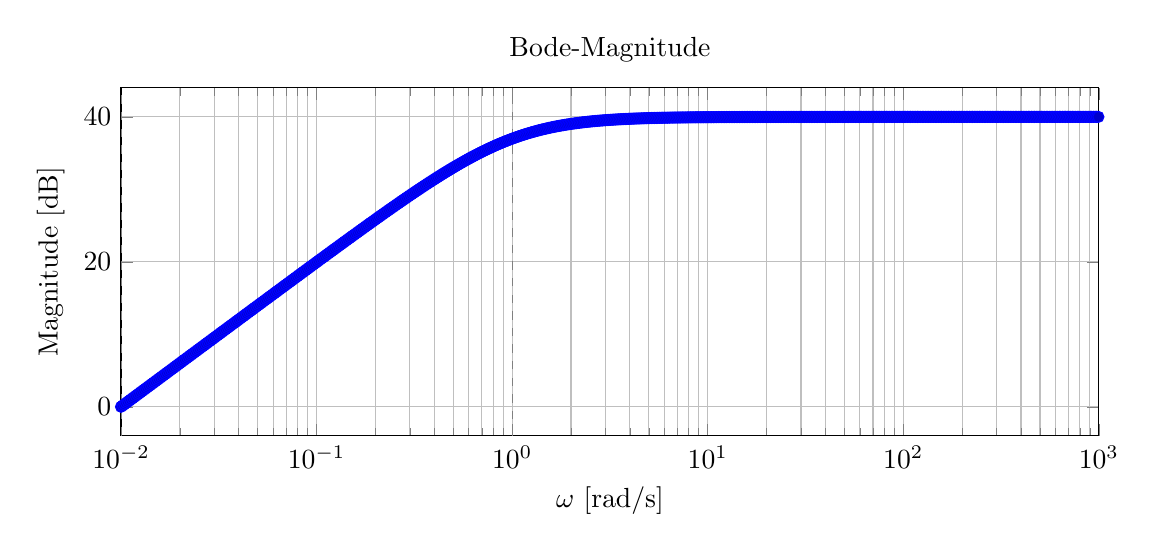
\begin{tikzpicture}
\begin{semilogxaxis}[
  width=14cm,height=6cm,
  xmin=1e-2,xmax=1e3,
  xlabel={$\omega$ [rad/s]},
  ylabel={Magnitude [dB]},
  grid=both,
  title={Bode-Magnitude}
]
\addplot+[domain=1e-2:1e3,samples=600] {40 + 20*log10(x) - 20*log10(sqrt(1 + x^2))};
\draw[gray,dashed] (rel axis cs:0,0) -- (rel axis cs:0,1);
\draw[gray,dashed] (axis cs:1,\pgfkeysvalueof{/pgfplots/ymin}) -- (axis cs:1,\pgfkeysvalueof{/pgfplots/ymax});
\node[gray,anchor=south east] at (axis cs:1,\pgfkeysvalueof{/pgfplots/ymax}) {\scriptsize Pol $\omega_p=1$};
\end{semilogxaxis}
\end{tikzpicture}

\vspace{6mm}

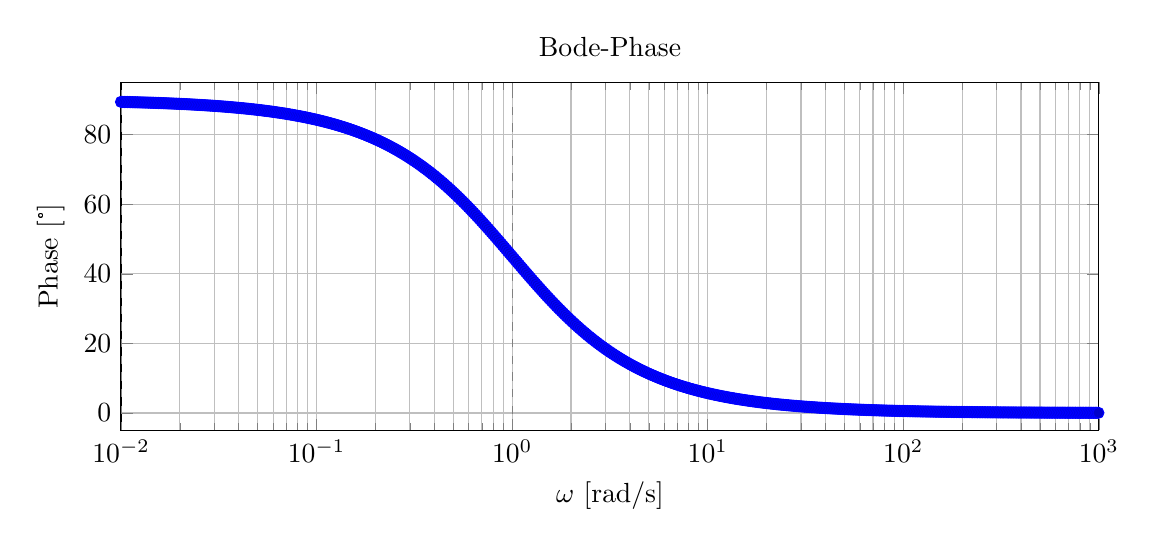
\begin{tikzpicture}
\begin{semilogxaxis}[
  width=14cm,height=6cm,
  xmin=1e-2,xmax=1e3,
  ymin=-5,ymax=95,
  xlabel={$\omega$ [rad/s]},
  ylabel={Phase [°]},
  grid=both,
  title={Bode-Phase}
]
\addplot+[domain=1e-2:1e3,samples=600] {90 - atan(x)};
\draw[gray,dashed] (rel axis cs:0,0) -- (rel axis cs:0,1);
\draw[gray,dashed] (axis cs:1,\pgfkeysvalueof{/pgfplots/ymin}) -- (axis cs:1,\pgfkeysvalueof{/pgfplots/ymax});
\node[gray,anchor=south east] at (axis cs:1,\pgfkeysvalueof{/pgfplots/ymax}) {\scriptsize Pol $\omega_p=1$};
\end{semilogxaxis}
\end{tikzpicture}
\end{center}

\subsection{Erklärung}
Nullstelle im Ursprung: Steigung $+20\,\mathrm{dB/dec}$ für kleine $\omega$ und Phasenbeitrag $\approx +90^\circ$. Pol bei $\omega_p=1\,\mathrm{rad/s}$: ab $\omega\gtrsim1$ Gesamtslope $\to 0\,\mathrm{dB/dec}$, Phase fällt von $+90^\circ$ gegen $0^\circ$ gemäß $90^\circ-\arctan(\omega)$. DC-Gewinn $100$ verschiebt die Magnitude um $+40\,\mathrm{dB}$; für $\omega\gg1$ nähert sich $|H(j\omega)|$ einer Konstanten bei etwa $40\,\mathrm{dB}$.
\end{document}